\subsection{Struktura podsystemu}
\label{subsec:cs-struktura}

\begin{figure}[ht]
    \leftskip-2em
    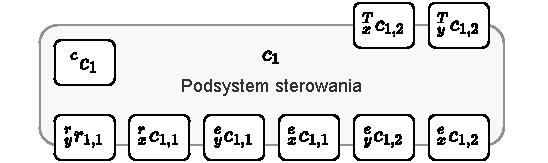
\includegraphics[width=1.15\columnwidth]{figures/ISR-cs-model.pdf}
    \caption{Struktura ogólna podsystemu sterowania}
    \label{fig:model-cs}
\end{figure}

Na rysunku~\ref{fig:model-cs} przedstawiono widok podsystemu sterowania w~systemie. Jego rolą w systemie jest nadzorowanie pracy pozostałych podsystemów oraz komunikacja z~innymi agentami. W~podsystemie celowo pominięto bufor do nadawania komunikatów do innych agentów, ponieważ zgodnie z~poleceniem, agent nie nadaje żadnych wiadomości do innych agentów. Krok dyskretyzacji podsystemu sterowania jest dostosowany do działania kamery i~wynosi ${}^{c}T = \frac{1}{30}$s.

\subsubsection{Pamięć wewnętrzna}
W~pamięci wewnętrznej podsystemu przechowywane są informacje na temat jego działania.
\begin{equation}
    {}^{c}c_{1,1} = [M, i, j, \Theta_{\mathrm{plan}}]
\end{equation}

\begin{itemize}
    \item $M$ -- macierz zer i~jedynek rozmiaru 20x20 opisująca zajętość palety,
    \item $i,j$ -- współrzędne rozważanego miejsca na palecie, numerowane od 1 do 20, 0 oznacza niewyznaczoną pozycję,
    \item $\Theta_{\mathrm{plan}}$ -- zmienna przechowująca zaplanowaną pozycję chwytu/odłożenia sześcianu.
\end{itemize}

Oprócz zmiennych, w~pamięci wewnętrznej przechowywane są stałe pozycje, służące do przygotowania systemu do chwytania i~odkładania.

\begin{itemize}
    \item $\Theta_{\mathrm{grip}}$ -- pozycja startowa do chwytu sześcianu, 
    \item $\Theta_{\mathrm{drop}}$ -- pozycja startowa do odkładania sześcianu.
\end{itemize}
    
\subsubsection{Bufory komunikacyjne}
Podsystem komunikuje się z~wirtualnymi efektorami, wirtualnymi receptorami oraz innymi agentami za pomocą następujących buforów komunikacyjnych.
\begin{itemize}
    \item ${}^{T}_{x}c_{2,1} = m \in \{ \emptyset, START \}$ -- komunikat od agenta $a_{2}$,
    
    \item ${}^{r}_{y}r_{1,1} = \varphi \in \{b, p\}$ -- wybór trybu pracy wirtualnego receptora kamery,
    \item ${}^{r}_{x}r_{1,1} = \Theta_{\mathrm{d}}$ -- znaleziona pozycja sześcianu/miejsca w~zależności od wybranego trybu,

    \item ${}^{e}_{y}e_{1,1} = \Theta_{\mathrm{zad}}$ -- zadana pozycja ramienia,
    \item ${}^{e}_{x}e_{1,1} = \Theta$ -- aktualna pozycja ramienia,

    \item ${}^{e}_{y}e_{1,2} = \xi_{\mathrm{zad}} \in \{o, c\}$ -- zadany stan chwytaka,
    \item ${}^{e}_{x}e_{1,2} = \xi \in \{o, c\}$ -- aktualny stan chwytaka.
\end{itemize}

\subsubsection{Funkcje pomocnicze}
Do poprawnego działania podsystemu, wymagana jest implementacja kilku funkcji pomocniczych, których konkretna definicja pozostaje poza zakresem projektu.

\begin{itemize}
    \item \texttt{zeros()} -- stwórz macierz 20x20 wypełnioną zerami,
    \item \texttt{ $isValid(\Theta)$ } -- sprawdza czy $\Theta$ jest poprawną pozycją znajdującą się w~przestrzeni operacyjnej robota,
    \item \texttt{makePlan($\Theta, \Theta_{\mathrm{d}}$)} -- na podstawie aktualnego położenia $\Theta$, wykrytego położenia $\Theta_{\mathrm{d}}$ oraz znanej prędkości taśmociągu, określa położenie w~którym robot złapie sześcian, 
    \item \texttt{findPlace($\Theta_{\mathrm{d}}, M$)} --na podstawie położeń wykrytych potencjalnych miejsc $\Theta_{\mathrm{d}}$ oraz znanej zajętości palety $M$, określa położenie w~którym robot odłoży sześcian,
    \item \texttt{isFull($M$)} -- sprawdza czy podana macierz zajętości palety jest wypełniona (czy należy zakończyć pracę).
\end{itemize}

\subsection{Automat sterujący}
\label{subsec:cs-automat}

\begin{figure}[ht]
    \leftskip-5em
    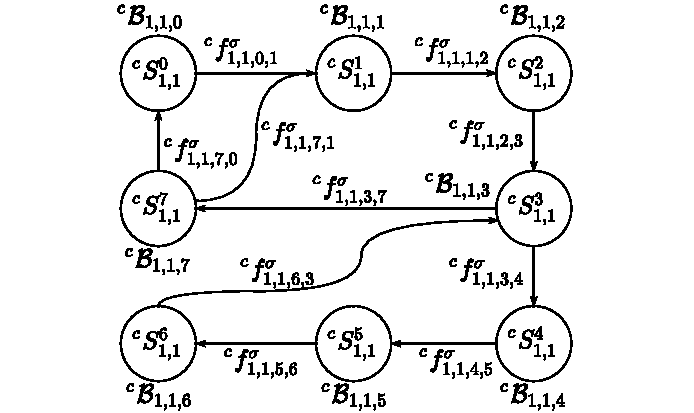
\includegraphics[ width=1.4\columnwidth]{figures/ISR-cs-behaviours.pdf}
    \caption{Automat zachowań podsystemu sterowania}
    \label{fig:zachowania-cs}
\end{figure}

Na rysunku~\ref{fig:zachowania-cs} przedstawiony został automat sterujący podsystemem sterowania. Z~każdym stanem $\{ {}^{c}S_{1,1}^0, \hdots, {}^{c}S_{1,1}^7 \}$ zostało skojarzone zachowanie $\{ {}^{c}\mathcal{B}_{1,1,0}, \hdots, {}^{c}\mathcal{B}_{1,1,7} \}$. Każdemu z~zachowań została nadana nazwa, w~celu uproszczenia dalszego opisu:
\begin{itemize}
    \item ${}^{c}\mathcal{B}_{1,1,0}$ - idle,
    \item ${}^{c}\mathcal{B}_{1,1,1}$ - pre-grip,
    \item ${}^{c}\mathcal{B}_{1,1,2}$ - detect-block,
    \item ${}^{c}\mathcal{B}_{1,1,3}$ - do-plan,
    \item ${}^{c}\mathcal{B}_{1,1,4}$ - grip,
    \item ${}^{c}\mathcal{B}_{1,1,5}$ - pre-store,
    \item ${}^{c}\mathcal{B}_{1,1,6}$ - detect-place,
    \item ${}^{c}\mathcal{B}_{1,1,7}$ - drop.
\end{itemize}

Dla stanów ${}^{c}S_{1,1}^{3}$ oraz ${}^{c}S_{1,1}^{7}$ należy zbadać rozłączność warunków początkowych stanów następnych tj. $\{ {}^{c}S_{1,1}^{4}, {}^{c}S_{1,1}^{7} \}$ i~$\{ {}^{c}S_{1,1}^{0}, {}^{c}S_{1,1}^{1} \}$. 
\medskip
\begin{equation}
    \begin{gathered}
        {}^{c}f^{\sigma}_{1,1,7,0} \land {}^{c}f^{\sigma}_{1,1,7,1} = False\\
        {}^{c}f^{\sigma}_{1,1,7,0} \lor {}^{c}f^{\sigma}_{1,1,7,1} = True \\
        \\
        {}^{c}f^{\sigma}_{1,1,3,4} \land {}^{c}f^{\sigma}_{1,1,3,7} = False\\
        {}^{c}f^{\sigma}_{1,1,3,4} \lor {}^{c}f^{\sigma}_{1,1,3,7} = True \\
    \end{gathered}
    \label{eqn:dowod}
\end{equation}
\medskip


Na podstawie~\ref{eqn:dowod}, stwierdzono rozłączność i~kompletność warunków początkowych stanów ${}^{c}S_{1,1}^{3}$ oraz ${}^{c}S_{1,1}^{7}$. Pozostałe stany mają tylko jeden warunek początkowy, co sprawia że nie ma potrzeby badać rozłączności oraz kompletności.

\subsection{Zachowanie idle}
\label{subsec:cs-idle}

Zachowanie ${}^{c}\mathcal{B}_{1,1,0}$, zwane dalej zachowaniem \textbf{idle}, jest pierwszym zachowaniem, które przejmuje kontrolę nad systemem. Jego celem jest oczekiwanie na komunikat \texttt{START} od agenta $a_{2}$.

\subsubsection{Funkcja przejścia}
\begin{equation}
{}^{c_{1,1}, c_{1,1}}f_{1,1,0} \triangleq {}^{c}c_{1,1} = [\text{\texttt{zeros()}}, 0, 0, \emptyset]  
\end{equation}

\begin{figure}[ht]
    \leftskip1.5em
    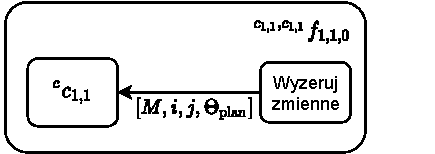
\includegraphics[width=\columnwidth]{figures/ISR-cs-fp-idle.pdf}
    \caption{Zdekomponowana funkcja przejścia zachowania \textbf{idle} w~postaci DFD}
    \label{fig:cs-fp-idle}
\end{figure}

\subsubsection{Warunki początkowe}
\begin{equation}
    {}^{c}f^{\sigma}_{1,1,7,0} \triangleq \Xi = o \land \text{\texttt{isFull($M$)}}
\end{equation}

\subsubsection{Warunki końcowe}
\begin{equation}
    {}^{c}f^{\tau}_{1,1,0} \triangleq {}^{T}_{x}c_{2,1} = \text{\texttt{START}}
\end{equation}

%%%%%%%%%%%%%%%%%%%%%%%%%%%%%%%%%%%%%%%%%%%%%%%%%%%%%%%%%%%%%%%%%%%%%%%%%%%%%%%%%%%%%

\subsection{Zachowanie pre-grip}
\label{subsec:cs-pre-grip}

Rolą zachowania ${}^{c}\mathcal{B}_{1,1,1}$ (\textbf{pre-grip}), jest przygotowanie systemu do złapania sześcianu. W~tym celu, ramię robota zostanie ustawione w~pozycji $\Theta_{\mathrm{grip}}$ w~której to kamera znajdzie się nad taśmociągiem, aby móc obserwować pojawiające się na nim sześciany. Dodatkowo, w~tym zachowaniu, podsystem sterowania wysyła komendy do chwytaka dwustanowego, aby otworzył swój uchwyt.

\subsubsection{Funkcja przejścia}
\begin{equation}
    \begin{gathered}
        {}^{c_{1,1}, e_{1,1}}f_{1,1,1} \triangleq {}^{e}_{y}c_{1,1} = \Theta_{\mathrm{grip}},
        \\
        {}^{c_{1,1}, e_{1,2}}f_{1,1,1} \triangleq {}^{e}_{y}c_{1,2} = o
    \end{gathered}
\end{equation}
    
\begin{figure}[ht]
    \leftskip2.5em
    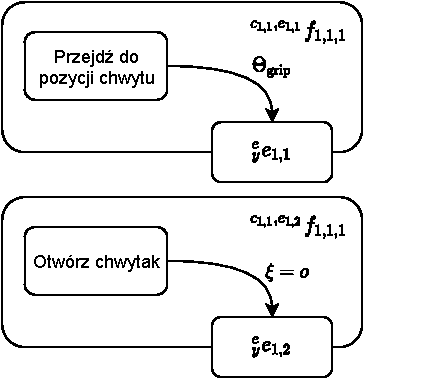
\includegraphics[width=\columnwidth]{figures/ISR-cs-fp-pre-grip.pdf}
    \caption{Zdekomponowana funkcja przejścia zachowania \textbf{pre-grip} w~postaci DFD}
    \label{fig:cs-fp-pre-grip}
\end{figure}

\subsubsection{Warunki początkowe}
\begin{equation}
    \begin{gathered}
        {}^{c}f^{\sigma}_{1,1,0,1} \triangleq {}^{T}_{x}c_{2,1} = START\\
        {}^{c}f^{\sigma}_{1,1,7,1} \triangleq \Xi = o \land \neg \text{\texttt{isFull($M$)}}
    \end{gathered}
\end{equation}

\subsubsection{Warunki końcowe}
\begin{equation}
    {}^{c}f^{\tau}_{1,1,1} \triangleq \Theta = \Theta_{\mathrm{grip}} \land \Xi = o
\end{equation}

%%%%%%%%%%%%%%%%%%%%%%%%%%%%%%%%%%%%%%%%%%%%%%%%%%%%%%%%%%%%%%%%%%%%%%%%%%%%%%%%%%%%%

\subsection{Zachowanie detect-block}
\label{subsec:cs-detect-block}
W~trakcie stanu aktywności zachowania ${}^{c}\mathcal{B}_{1,1,2}$ (\textbf{detect-block}), robot obserwuje taśmociąg, na którym pojawiają się kolorowe sześciany. Funkcja przejścia oczekuje aż wirtualny receptor, który przetwarza obraz z~kamery, zwróci poprawną pozycję wykrytego, żółtego sześcianu i~na tej podstawie oraz znajomości prędkości taśmociągu, określa pozycję w~której dojdzie do chwytu.

\subsubsection{Funkcja przejścia}
\begin{equation}
    \begin{gathered}
      {}^{c_{1,1}, r_{1,1}}f_{1,1,2} \triangleq {}^{r}_{y}c_{1,1} = b\\        
      {}^{c_{1,1}, c_{1,1}}f_{1,1,2} \triangleq \\ \Theta_{\mathrm{plan}} =
                   \begin{cases}
       			    \text{\texttt{makePlan($\Theta, \Theta_{\mathrm{d}}$)}}, & \text{\texttt{isValid($\Theta_{\mathrm{d}}$)}}\\
                       \emptyset, & \text{w p.p.}
       		    \end{cases}
    \end{gathered}
\end{equation}

\begin{figure}[ht]
    \leftskip1.5em
    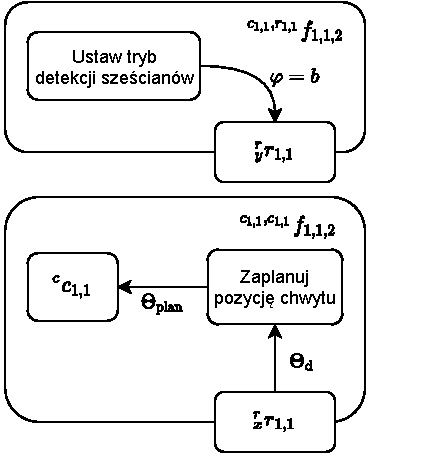
\includegraphics[width=\columnwidth]{figures/ISR-cs-fp-detect-block.pdf}
    \caption{Zdekomponowana funkcja przejścia zachowania \textbf{detect-block} w~postaci DFD}
    \label{fig:cs-fp-detect-block}
\end{figure}

\subsubsection{Warunki początkowe}
\begin{equation}
    {}^{c}f^{\sigma}_{1,1,1,2} \triangleq {}^{c}f^{\tau}_{1,1,1} = True
\end{equation}

\subsubsection{Warunki końcowe}
\begin{equation}
    {}^{c}f^{\tau}_{1,1,2} \triangleq \text{\texttt{isValid($\Theta_{\mathrm{d}}$)}}
\end{equation}


%%%%%%%%%%%%%%%%%%%%%%%%%%%%%%%%%%%%%%%%%%%%%%%%%%%%%%%%%%%%%%%%%%%%%%%%%%%%%%%%%%%%%

\subsection{Zachowanie do-plan}
\label{subsec:cs-do-plan}
Zachowanie ${}^{c}\mathcal{B}_{1,1,3}$ (\textbf{do-plan}), realizuje wcześniej wygenerowany plan $\Theta_{plan}$, który został zapisany w~pamięci wewnętrznej podsystemu.

\subsubsection{Funkcja przejścia}
\begin{equation}
    {}^{c_{1,1}, e_{1,1}}f_{1,1,3} \triangleq {}^{e}_{y}c_{1,1} = \Theta_{\mathrm{plan}}
\end{equation}

\begin{figure}[ht]
    \leftskip1.5em
    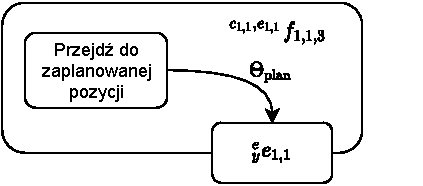
\includegraphics[width=\columnwidth]{figures/ISR-cs-fp-do-plan.pdf}
    \caption{Zdekomponowana funkcja przejścia zachowania \textbf{do-plan} w~postaci DFD}
    \label{fig:cs-fp-do-plan}
\end{figure}

\subsubsection{Warunki początkowe}
\begin{equation}
    \begin{gathered}
        {}^{c}f^{\sigma}_{1,1,2,3} \triangleq \text{\texttt{isValid($\Theta_{\mathrm{d}}$)}} = True \\
        {}^{c}f^{\sigma}_{1,1,6,3} \triangleq \text{\texttt{isValid($\Theta_{\mathrm{d}}$)}} = True        
    \end{gathered}
\end{equation}

\subsubsection{Warunki końcowe}
\begin{equation}
    {}^{c}f^{\tau}_{1,1,3} \triangleq \Theta = \Theta_{\mathrm{plan}}
\end{equation}


%%%%%%%%%%%%%%%%%%%%%%%%%%%%%%%%%%%%%%%%%%%%%%%%%%%%%%%%%%%%%%%%%%%%%%%%%%%%%%%%%%%%%

\subsection{Zachowanie grip}
\label{subsec:cs-grip}
W~trakcie zachowania ${}^{c}\mathcal{B}_{1,1,4}$, chwytak robota łapie wykryty klocek.R
System oczekuje na moment w~którym klocek znajdzie się w~przewidywanej pozycji, trzymając chwytak w~gotowości. Chwytak zaciska się w~momencie gdy wykryta pozycja klocka znajdzie się pomiędzy jego palcami. Zachowanie kończy się w~momencie uzyskania informacji o~uzyskaniu maksymalnego zamknięcia chwytaka.

\subsubsection{Funkcja przejścia}
\begin{equation}
    {}^{c_{1,1}, e_{1,2}}f_{1,1,4} \triangleq {}^{e}_{y}c_{1,2} = \begin{cases}
        c, & \Theta_{\mathrm{plan}} = \Theta_{\mathrm{d}}\\
        o, & \Theta_{\mathrm{plan}} \neq \Theta_{\mathrm{d}}
    \end{cases}
\end{equation}

\begin{figure}[ht]
    \leftskip1.5em
    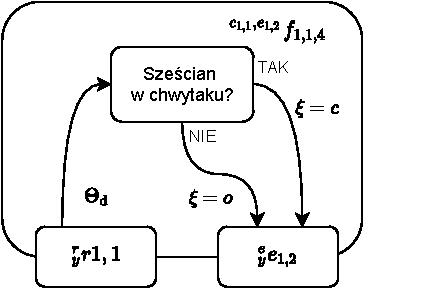
\includegraphics[width=\columnwidth]{figures/ISR-cs-fp-grip.pdf}
    \caption{Zdekomponowana funkcja przejścia zachowania \textbf{grip} w~postaci DFD}
    \label{fig:cs-fp-grip}
\end{figure}

\subsubsection{Warunki początkowe}
\begin{equation}
    {}^{c}f^{\sigma}_{1,1,3,4} \triangleq {}^{c}f^{\tau}_{1,1,3} = True \land \Xi = o
\end{equation}

\subsubsection{Warunki końcowe}
\begin{equation}
    {}^{c}f^{\tau}_{1,1,4} \triangleq \Xi = c
\end{equation}

%%%%%%%%%%%%%%%%%%%%%%%%%%%%%%%%%%%%%%%%%%%%%%%%%%%%%%%%%%%%%%%%%%%%%%%%%%%%%%%%%%%%%

\subsection{Zachowanie pre-drop}
\label{subsec:cs-pre-drop}
Zachowanie ${}^{c}\mathcal{B}_{1,1,5}$ (\textbf{pre-drop}) jest bliźniaczo podobne do zachowania~\textbf{pre-grip}, jednak różni się pozycją docelową. Dodatkowo, w~trakcie jego aktywności, robot cały czas musi trzymać sześcian w~chwytaku. Pozycja robota $\Theta_{\mathrm{drop}}$ została tak przygotowana, aby robot mógł bez problemu obserwować całą paletę do składowania sześcianów.

\subsubsection{Funkcja przejścia}
\begin{equation}
    {}^{c_{1,1}, e_{1,1}}f_{1,1,5} \triangleq {}^{e}_{y}c_{1,1} = \Theta_{\mathrm{drop}}
\end{equation}

\begin{figure}[ht]
    \leftskip1.5em
    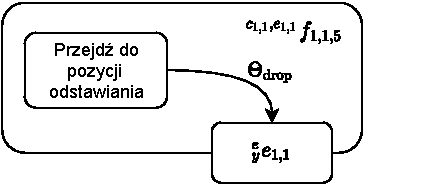
\includegraphics[width=\columnwidth]{figures/ISR-cs-fp-pre-drop.pdf}
    \caption{Zdekomponowana funkcja przejścia zachowania \textbf{pre-drop} w~postaci DFD}
    \label{fig:cs-fp-pre-drop}
\end{figure}

\subsubsection{Warunki początkowe}
\begin{equation}
    {}^{c}f^{\sigma}_{1,1,4,5} \triangleq \Xi = c
\end{equation}

\subsubsection{Warunki końcowe}
\begin{equation}
    {}^{c}f^{\tau}_{1,1,5} \triangleq \Theta = \Theta_{\mathrm{drop}}
\end{equation}

%%%%%%%%%%%%%%%%%%%%%%%%%%%%%%%%%%%%%%%%%%%%%%%%%%%%%%%%%%%%%%%%%%%%%%%%%%%%%%%%%%%%%

\subsection{Zachowanie detect-place}
\label{subsec:cs-detect-place}
Zachowanie ${}^{c}\mathcal{B}_{1,1,6}$ (\textbf{detect-place}) jest odpowiednikiem zachowania \textbf{detect-block}, z~tą różnicą że w~trakcie jego aktywności wykrywane są docelowe miejsca na odłożenie. Na tej podstawie wybierane jest konkretne miejsce na palecie (współrzędne $i,j$) oraz plan operacji $\Theta_{plan}$.

\subsubsection{Funkcja przejścia}
\begin{equation}
    \begin{gathered}
        {}^{c_{1,1}, r_{1,1}}f_{1,1,6} \triangleq {}^{r}_{y}c_{1,1} = p\\
        {}^{c_{1,1}, c_{1,1}}f_{1,1,6} \triangleq \\ [\Theta_{\mathrm{plan}}, i, j] =
            \begin{cases}
			    \text{\texttt{findPlace($\Theta, \Theta_{\mathrm{d}}, M$)}}, & \text{\texttt{isValid($\Theta_{\mathrm{d}}$)}}\\
                [\emptyset, 0, 0], & \text{w p.p.}
		    \end{cases}
    \end{gathered}
\end{equation}

\begin{figure}[ht]
    \leftskip1.5em
    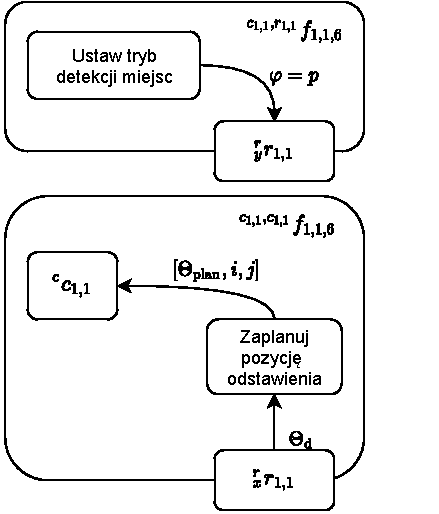
\includegraphics[width=\columnwidth]{figures/ISR-cs-fp-detect-place.pdf}
    \caption{Zdekomponowana funkcja przejścia zachowania \textbf{detect-place} w~postaci DFD}
    \label{fig:cs-fp-detect-place}
\end{figure}

\subsubsection{Warunki początkowe}
\begin{equation}
    {}^{c}f^{\sigma}_{1,1,5,6} \triangleq {}^{c}f^{\tau}_{1,1,5} = True
\end{equation}

\subsubsection{Warunki końcowe}
\begin{equation}
    {}^{c}f^{\tau}_{1,1,6} \triangleq \text{\texttt{isValid($\Theta_{\mathrm{d}}$)}}
\end{equation}

%%%%%%%%%%%%%%%%%%%%%%%%%%%%%%%%%%%%%%%%%%%%%%%%%%%%%%%%%%%%%%%%%%%%%%%%%%%%%%%%%%%%%

\subsection{Zachowanie drop}
\label{subsec:cs-drop}
Ostatnim rozważanym zachowaniem w~podsystemie sterowania jest ${}^{c}\mathcal{B}_{1,1,6}$ (\textbf{drop}), podczas którego robot uwalnia sześcian ze swojego uchwytu, zostawiając go w~zaplanowanym miejscu. Robot odznacza w~pamięci, które komórki palety zostały zajęte, dzięki czemu możliwe jest stwierdzenie czy zadanie zostało zakończone oraz w~przeciwnym przypadku, umożliwia dalsze planowanie czynności.

\subsubsection{Funkcja przejścia}
\begin{equation}
    \begin{gathered}
        {}^{c_{1,1}, c_{1,1}}f_{1,1,7} \triangleq M[i,j] = 1 \\
        {}^{c_{1,1}, e_{1,2}}f_{1,1,7} \triangleq {}^{e}_{y}c_{1,2} = o
    \end{gathered}
\end{equation}

\begin{figure}[ht]
    \leftskip1em
    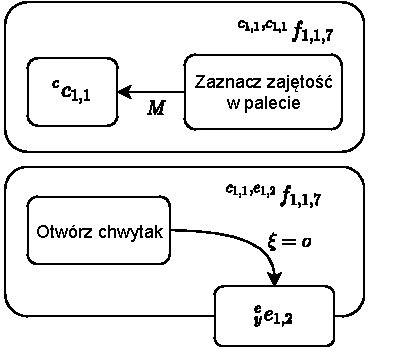
\includegraphics[width=\columnwidth]{figures/ISR-cs-fp-drop.pdf}
    \caption{Zdekomponowana funkcja przejścia zachowania \textbf{drop} w~postaci DFD}
    \label{fig:cs-fp-drop}
\end{figure}

\subsubsection{Warunki początkowe}
\begin{equation}
    {}^{c}f^{\sigma}_{1,1,3,7} \triangleq {}^{c}f^{\tau}_{1,1,3} = True \land \Xi = c
\end{equation}

\subsubsection{Warunki końcowe}
\begin{equation}
    {}^{c}f^{\tau}_{1,1,7} \triangleq \Xi = o
\end{equation}
